% IE 643: Deep Learning - Theory and Practice, July-Dec 2026
% Project Report - Team DeX
% Compile:  pdflatex IE643_Project_Report_DeX.tex  (twice, for references)
\documentclass[11pt,a4paper]{article}

\usepackage[margin=1in]{geometry}
\usepackage{amsmath,amssymb}
\usepackage{booktabs}
\usepackage{graphicx}
\usepackage{xcolor}
\usepackage{array}
\usepackage{caption}
\usepackage{enumitem}
\usepackage{tikz}
\usetikzlibrary{arrows.meta,positioning,shapes.geometric,fit,backgrounds}
\usepackage[colorlinks=true,linkcolor=blue,citecolor=teal,urlcolor=blue]{hyperref}

\captionsetup{font=small,labelfont=bf}
\setlength{\parskip}{0.5em}
\setlength{\parindent}{0pt}
\newcommand{\code}[1]{\texttt{\small #1}}

\begin{document}

%% ------------------------------------------------------------------ title box
\begin{center}
\fbox{\begin{minipage}{0.95\textwidth}
\vspace{2mm}
{\bfseries IE 643: Deep Learning - Theory and Practice} \hfill {\bfseries July-Dec 2026}\\[2mm]
\begin{center}
{\Large Project Report: Cross-Template Key-Value Field Extraction\\[1mm]
from Scanned Forms}
\end{center}
\vspace{1mm}
{\itshape Team Name: DeX} \hfill {\itshape Team Members: 26M1510 (Mudiam Naga Sukesh)}
\vspace{2mm}
\end{minipage}}
\end{center}

\vspace{6mm}

%% -------------------------------------------------------------------- abstract
\begin{center}
\begin{minipage}{0.86\textwidth}
\begin{center}\textbf{Abstract}\end{center}
\small
This report describes a document-understanding system that extracts key-value fields from
scanned forms and is evaluated on form templates for which it has seen \emph{zero} training
examples. The task is posed without a schema: rather than being told which fields to look for,
the model tags every word with a role (key, value, header or none) and then decides, for each
value, which key on the page it answers. Both decisions are made by two small heads on a shared LayoutLMv3 backbone that reads the words,
their boxes and the page image, trained jointly with a tagging loss and a per-value softmax
linking loss.
The central design choice is that the linking head sees geometry only as \emph{relative}
offsets in a scale-invariant frame, which we prove is invariant to translation and scaling of
the page, and which an ablation shows is what makes the representation transfer. Training uses
FUNSD, SROIE and WildReceipt under a template-level split with explicit leakage assertions;
VRDU is held out entirely and never trained on. On unseen templates the final system reaches
0.713 value recall against 0.928 on seen templates, and under VRDU's own benchmark-style field
metric scores 0.541 micro F1 on registration forms and 0.538 unrepeated F1 on ad-buy forms, with
no VRDU training data at all. The page-image stream is switched on in the final system. Against
the otherwise identical text-and-layout model it raises unseen value recall (0.695 to 0.713) and
ad-buy F1 (0.497 to 0.538) but lowers registration-form F1 (0.593 to 0.541); each is a single run,
so the report claims a direction and not a significant difference. A second split that holds out
in-domain templates, measured on the text-and-layout model, shows that entity, link and
end-to-end pair F1 do \emph{not} degrade on unseen templates --- every gap interval contains zero
--- establishing that the headline gap is domain shift rather than template novelty. A failure
analysis isolates the two structural assumptions that break: that a key sits beside its
value, and that every value carries a printed label.
\end{minipage}
\end{center}

\vspace{4mm}

%% ==================================================================== 1. INTRO
\section{Introduction}

Organisations receive the same information on endlessly different pieces of paper. A purchase
order, an invoice, a government registration statement and a broadcast advertising contract all
carry fields such as a date, a party's name and an amount, but each lays them out differently.
The practical cost of this is that document-extraction systems are usually built
\emph{per template}: somebody collects examples of a form, annotates them, and trains or
configures a model for that form. The moment a new layout arrives --- a different vendor, a
revised version of the same government form --- the process repeats.

This project asks whether that per-template cost can be avoided. Concretely: can a model learn,
from a set of training templates, a representation of text, layout and spatial relationships
general enough that it extracts key-value fields correctly from a template it has never seen,
with no labelled or unlabelled data from that template used at any point in training?

The question matters because the alternative scales badly, and because it is a clean test of
what a document model has actually learned. A model that memorises ``the invoice number is in
the top right'' will score well on a held-out \emph{document} of a template it trained on and
fail on a new layout. Only a template-level split can tell these apart, and most reported
numbers in this area do not use one.

Our answer has three parts. First, we pose the task \textbf{schema-free}: the model is never
given a list of field names, so it cannot overfit to a fixed vocabulary of fields and can
therefore be asked about forms whose fields it has never heard of. Second, we make the
representation \textbf{geometrically relative}: the component that decides which key a value
answers sees only offsets between the two boxes, measured in units of the page's own text size,
and we prove this is invariant to where the form sits on the page and how large it is scanned.
Third, we measure \textbf{honestly}: splits are built over induced templates with leakage
assertions that fail loudly, confidence intervals resample templates rather than documents, and
metrics that a dataset cannot support are reported as not-measurable rather than as zero.

\textbf{Structure of this report.} Section~\ref{sec:workflow} outlines the project workflow.
Section~\ref{sec:lit} surveys the material we reviewed. Section~\ref{sec:approach} describes the
proposed approach, split into the work done before the prep-presentation review
(Section~\ref{sec:before}) and after it (Section~\ref{sec:after}). Section~\ref{sec:data} gives
the dataset details. Section~\ref{sec:exp} describes every experiment performed, including those
with negative results. Section~\ref{sec:results} presents the results.
Section~\ref{sec:novelty} gives the plan for novelty assessment, and
Section~\ref{sec:conclusion} concludes.

\begin{sloppypar}
\textbf{Code and trained models.} The complete source, configuration and this report are at
\url{https://github.com/MudiamSukesh/cross-template-kv-extraction}. The four trained
checkpoints are published as release assets at
\url{https://github.com/MudiamSukesh/cross-template-kv-extraction/releases/tag/v1.0}.
\end{sloppypar}

%% ================================================================= 2. WORKFLOW
\section{Project Workflow}
\label{sec:workflow}

\begin{itemize}[leftmargin=1.4em,itemsep=2pt]
  \item \textbf{Problem framing.} Fix the task as cross-template key-value extraction with zero
        same-template training data; identify that a template-level split is the only valid
        evaluation.
  \item \textbf{First attempt (pre-review).} A schema-driven, query-based extractor: supply a
        field name as a query, have the model tag the span answering it. Abandoned; see
        Section~\ref{sec:before}.
  \item \textbf{Restart (post-review).} Re-pose the task schema-free as tag-and-link, with two
        heads on one backbone.
  \item \textbf{Data curation.} Four public corpora into one unified page-level schema; a
        validator that refuses malformed records; an alignment check that verifies boxes sit on
        printed ink.
  \item \textbf{Template induction and splitting.} Cluster documents into templates by layout
        signature, then split \emph{templates} (not documents) into train, validation, seen test
        and unseen test, with leakage assertions.
  \item \textbf{Modelling.} LayoutLMv3 backbone with its page-image stream enabled; a BIO role tagger; a link scorer using relative
        geometry; joint training with two losses.
  \item \textbf{Evaluation.} Seen-versus-unseen gap with template-level bootstrap intervals;
        VRDU's own benchmark-style field scoring; per-field and per-source breakdowns.
  \item \textbf{Failure analysis.} Counterfactual layout probes and structural bucketing to name
        the assumptions that fail rather than merely reporting that they do.
  \item \textbf{Ablations.} One configuration key each, to test whether the generalisation
        techniques earn their place.
  \item \textbf{Interface.} A web application that accepts an uploaded image or PDF, runs OCR and
        the model, and draws the extracted pairs on the page.
\end{itemize}

\begin{figure}[htbp]
\centering
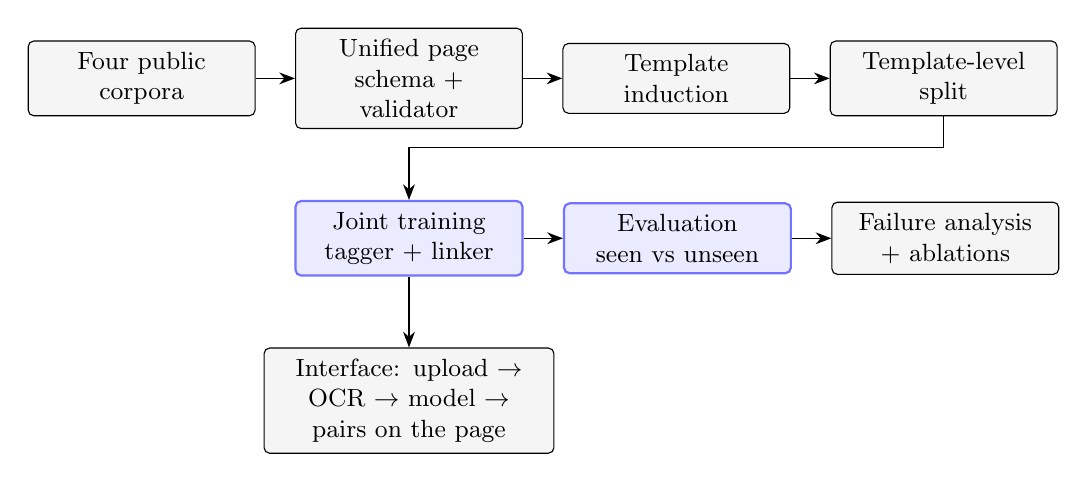
\begin{tikzpicture}[
  node distance=5mm,
  box/.style={draw,rounded corners=2pt,align=center,inner sep=4pt,font=\small,
              minimum height=8mm,text width=26mm},
  lit/.style={box,fill=blue!8,draw=blue!55,thick},
  dat/.style={box,fill=black!4},
  >={Stealth[length=2mm]}
]
\node[dat] (raw)  {Four public\\corpora};
\node[dat,right=of raw] (uni) {Unified page\\schema + validator};
\node[dat,right=of uni] (tpl) {Template\\induction};
\node[dat,right=of tpl] (spl) {Template-level\\split};

\node[lit,below=9mm of uni] (train) {Joint training\\tagger + linker};
\node[lit,right=of train] (eval) {Evaluation\\seen vs unseen};
\node[dat,right=of eval] (fail) {Failure analysis\\+ ablations};

\node[dat,below=9mm of train,text width=34mm] (ui) {Interface: upload $\rightarrow$ OCR $\rightarrow$ model $\rightarrow$ pairs on the page};

\draw[->] (raw)--(uni); \draw[->] (uni)--(tpl); \draw[->] (tpl)--(spl);
\draw[->] (spl.south) -- ++(0,-4mm) -| (train.north);
\draw[->] (train)--(eval); \draw[->] (eval)--(fail);
\draw[->] (train.south) -- (ui.north);
\end{tikzpicture}
\caption{Project workflow. Shaded boxes are the two learned stages; everything else is data
preparation or measurement. VRDU enters only at the evaluation stage and never at training.}
\label{fig:workflow}
\end{figure}

%% =============================================================== 3. LIT SURVEY
\section{Literature Survey}
\label{sec:lit}

We restrict this survey to the material the project directly builds on.

\textbf{Layout-aware pre-trained backbones.} The LayoutLM family established that a transformer
over document text can be made layout-aware by adding the token's bounding box as a positional
input. LayoutLM~\cite{layoutlm} added 2D position embeddings to BERT. LayoutLMv2~\cite{layoutlmv2}
added a visual stream and a spatial-aware self-attention bias. LayoutLMv3~\cite{layoutlmv3}
simplified the recipe with unified text and image masking and word-patch alignment, and is the
backbone we use. The property we rely on is that the model consumes a sequence of
(token, box) pairs and produces contextual embeddings in which a word's neighbours on the
\emph{page} influence it, not only its neighbours in reading order. We note the detail that each
box coordinate is normalised to $[0, 1000]$ against the page's own width and height
independently, which distorts aspect ratio --- a point that motivates our own geometry handling
in Section~\ref{sec:geom}.

\textbf{Form-understanding datasets.} FUNSD~\cite{funsd} is the reference dataset for the task
we solve: 199 noisy scanned forms annotated with entities typed as question, answer or header,
\emph{and} with explicit links between them. It is the only corpus we use that supervises the
linking decision directly. SROIE~\cite{sroie} provides 973 scanned receipts with four extracted
field values per receipt but no key annotations and no links, which makes it value-only
supervision. WildReceipt~\cite{sdmgr} contributes 1{,}740 receipt images with 25 key-information
categories paired as \code{X\_key}/\code{X\_value}, from which links can be derived.

\textbf{The cross-template benchmark.} VRDU~\cite{vrdu} is the work closest to our problem
statement. It argues that existing benchmarks overstate generalisation because their train and
test documents share templates, and it supplies two corpora --- a registration-form corpus
derived from US FARA filings and an ad-buy-form corpus derived from the DeepForm project ---
together with explicit few-shot splits in which the test documents come from templates
\emph{unseen} during training. It also defines a careful field-matching protocol in which the
comparison between an extracted string and a gold one is type-specific: dates are compared after
parsing, prices within a tolerance, addresses under an edit-distance threshold, and so on. We
adopt both the corpora and this matching protocol, porting the published matching and scoring
code so that our numbers are comparable in kind to those reported there. Crucially, VRDU
annotates \emph{values only}: it does not mark which printed text on the page is the key, nor
link keys to values. This shapes what we can and cannot measure, as Section~\ref{sec:metrics}
explains.

\textbf{OCR.} Uploaded documents arrive as pixels, so the system needs its own text detection and
recognition. We use docTR~\cite{doctr} with the FAST detector~\cite{fast} and the
PARSeq~\cite{parseq} recogniser. PARSeq's permuted autoregressive formulation gives notably
better recognition on the short, noisy strings typical of scanned forms than the CRNN baseline
docTR falls back to, which is why the system verifies its weights are present and says so in the
interface when they are not.

%% ================================================================ 4. APPROACH
\section{Proposed Approach}
\label{sec:approach}

\subsection{Work done before prep-presentation review}
\label{sec:before}

The first design was \textbf{schema-driven and query-based}. A field name --- say
\code{signer\_name} --- was embedded as a query prepended to the page's tokens, and the model
tagged the span of words that answered that query, allowing multiple spans per query and up to
400 candidates. The backbone was LayoutLMv3-base, as it remains. A candidate-pruning stage
reduced the span search space before scoring, and the tag head used focal loss to counter the
severe class imbalance between answer words and the rest of the page.

This design was implemented, trained through several iterations and evaluated. It was then
\textbf{abandoned}, for reasons that are themselves a result and are reported in
Section~\ref{sec:negative}. In brief: the tag head collapsed on unseen templates, scoring 0.019
on the FARA corpus, the pruning stage capped achievable recall at 0.822 regardless of what the
model did downstream, and the per-query formulation could not resolve the common case of several
instances of the same field type on one page --- three different names on a single form, all
plausible answers to a query for ``name''. A proposed fix was to anchor each query to the
\emph{bounding box} of the printed key rather than supplying the key as text alone, turning the
question from ``what is the value called name?'' into ``what is the value of the entity at this
location?''. That idea survives, in a different form, as the link head of the current design.

The deeper problem was structural. A query-based model must be told what to ask for, which
re-introduces exactly the per-template, per-schema configuration cost that the project exists to
remove. At the review it was clear the approach had become complicated without addressing the
central question, and the decision was taken to restart.

\subsection{Work done after prep-presentation review}
\label{sec:after}

The system was re-posed \textbf{schema-free}. The model is never told which fields exist. It
answers two questions about a page, and the deliverable is whatever key-value pairs the page
itself contains.

\subsubsection{Formulation}

\textbf{Head 1 --- role tagging.} Every word is assigned one of seven BIO tags: \code{O}, plus
\code{B-} and \code{I-} for each of KEY, VALUE and HEADER. A single linear layer maps the
backbone's hidden state $h_t$ of a word's first sub-token to tag logits,
\[
  z_t = W h_t + b, \qquad W \in \mathbb{R}^{7 \times 768},
\]
and spans are decoded by walking the sequence. Decoding is deliberately lenient: an \code{I-X}
with no open span opens a new one rather than being discarded, because a stray \code{I-} without
its \code{B-} is a common small error and recovering a span from it loses less than throwing the
word away.

\textbf{Head 2 --- linking.} Given the key spans and value spans on a page, the model decides
which key each value answers. A span's embedding is the mean of its words' hidden states,
$\bar h_k$ and $\bar h_v$, projected to a smaller entity space. The score of pairing key $k$ with
value $v$ is
\[
  s(k, v) \;=\; \mathrm{MLP}\!\left(\left[\, e_k \;;\; e_v \;;\; e_k \odot e_v \;;\;
  \varphi\big(g(k,v)\big) \,\right]\right),
\]
where $e_k, e_v$ are the projected span embeddings, $e_k \odot e_v$ is their elementwise product
(an interaction term that lets the model detect agreement between the two, which a concatenation
alone cannot express), and $\varphi(g(k,v))$ is a learned embedding of the twelve relative
geometry features of Section~\ref{sec:geom}. A separate scalar
\[
  n(v) \;=\; w_n^{\top} e_v + b_n
\]
scores the hypothesis that $v$ answers \emph{no} key on this page. For each value, the scores of
all candidate keys together with $n(v)$ form a softmax:
\[
  p(k \mid v) \;=\;
  \frac{\exp\big(s(k,v)\big)}{\exp\big(n(v)\big) + \sum_{k' \in K} \exp\big(s(k',v)\big)}.
\]
This is a per-value competition, which is the right shape for the data: one key may answer many
values (a column header above a column), but a value answers at most one key.

\subsubsection{The two losses}

Training minimises
\[
  \mathcal{L} \;=\; \mathcal{L}_{\text{tag}} \;+\; \lambda\, \mathcal{L}_{\text{link}},
  \qquad \lambda = 1 .
\]
The tagging loss is the mean cross-entropy over \emph{supervised} words only,
\[
  \mathcal{L}_{\text{tag}} \;=\; -\frac{1}{|S|}\sum_{t \in S} \log p\big(y_t = c_t \mid x\big),
\]
where $S$ excludes padding, non-first sub-tokens, words in \code{Ignore} segments, and --- for
value-only corpora such as SROIE and VRDU --- every word that is not part of an annotated value,
since on those pages we do not know whether any \emph{other} word is a key.

The linking loss treats the gold key set $G(v)$ of a value as a set of acceptable answers and
maximises their total probability:
\[
  \ell(v) \;=\; -\log \sum_{k \in G(v)} p(k \mid v),
\]
computed with \code{logsumexp} for numerical stability. Values whose gold key falls in a
different chunk are skipped rather than being scored as errors with an unreachable target.

\subsubsection{Relative geometry, and why it is the load-bearing idea}
\label{sec:geom}

LayoutLMv3 normalises each box coordinate to $[0,1000]$ against the page's width and height
\emph{separately}. A square stamp on a portrait page therefore becomes a non-square box, and the
same form scanned at a different size or offset produces different numbers. If the link head saw
those coordinates, it could learn ``the value is at $x \approx 700$'', which is true of the
training templates and false of everything else.

So the link head never sees absolute coordinates. It sees twelve features computed in an
aspect-preserving frame (the longest page side mapped to 1000, the other scaled by the same
factor) and expressed in units of the page's \emph{median word height} $m$: horizontal and
vertical centre offsets, the gap between the boxes, their width and height ratios, horizontal and
vertical overlap fractions, and indicators of reading-order direction. Each unbounded offset is
compressed by a signed log,
\[
  \operatorname{slog}(x) \;=\; \operatorname{sign}(x)\,\log\big(1 + |x|\big),
\]
which keeps a one-word gap and a half-page gap on the same scale without discarding the sign.

\textbf{Invariance.} Let a page be transformed by a translation and a uniform scaling,
$x' = \alpha x + \beta_x$ and $y' = \alpha y + \beta_y$. Any centre difference becomes
\[
  \Delta x' \;=\; (\alpha x_k + \beta_x) - (\alpha x_v + \beta_x) \;=\; \alpha\,\Delta x ,
\]
so the translation cancels. The median word height transforms as $m' = \alpha m$, so each feature,
being a ratio of a length to $m$, satisfies
\[
  \frac{\Delta x'}{m'} \;=\; \frac{\alpha\, \Delta x}{\alpha\, m} \;=\; \frac{\Delta x}{m} .
\]
Overlap fractions and aspect ratios are already dimensionless and likewise unchanged. The twelve
features are therefore \emph{identical} for a form photographed close up and the same form scanned
small in a corner, which is exactly the nuisance variation that distinguishes one template's
rendering from another's. Section~\ref{sec:ablations} shows this is not merely a nice property:
replacing it with absolute geometry improves seen-template accuracy and measurably destroys
cross-template transfer.

\subsubsection{Adaptation method}

The adaptation technique is \textbf{full fine-tuning} --- every one of the 126.0M backbone
parameters is updated, alongside 0.70M parameters in the two heads --- rather than LoRA, adapters
or a frozen backbone. Full fine-tuning was chosen because the task changes what the
\emph{representation} must encode (spatial relationships between entities, not just token
semantics), and a frozen backbone cannot adapt its attention to that. The risk of full
fine-tuning on a small corpus is memorisation of the training templates, so it is constrained by
five safeguards, listed in Table~\ref{tab:safeguards}.

\begin{table}[htbp]
\centering\small
\begin{tabular}{@{}p{3.5cm}p{9.9cm}@{}}
\toprule
\textbf{Safeguard} & \textbf{Why} \\
\midrule
Split learning rates & $3\times10^{-5}$ backbone, $3\times10^{-4}$ heads: the pre-trained weights
are good and should move slowly; the randomly initialised heads must move fast. \\
Warmup then linear decay & 10\% warmup stops large early updates from destroying pre-trained
features before the heads produce a useful signal. \\
AdamW, weight decay 0.01 & Excluding biases and LayerNorm parameters, which should not be
shrunk toward zero. \\
Gradient clipping at 1.0 & Caps the damage of any single bad batch. \\
Early stopping on validation \emph{templates} & Patience 5 on a mean of the validation metrics;
``best'' means best on layouts not trained on, so the stopping criterion itself rewards
generalisation. \\
\bottomrule
\end{tabular}
\caption{The five constraints placed on full fine-tuning.}
\label{tab:safeguards}
\end{table}

Geometric augmentation is applied during training: a global scale in $[0.85, 1.0]$, a random
shift, and per-word jitter of 0.15 word heights. The intent is to prevent the \emph{tagger} ---
which, unlike the link head, does see LayoutLMv3's absolute coordinates --- from memorising
positions.

\textbf{The page image: used by the final model.} LayoutLMv3 is a multimodal backbone, and the
delivered configuration (\code{runs\textbackslash visual}, \code{model.visual=true}) runs its image
stream. Besides \code{input\_ids}, \code{bbox} and \code{attention\_mask}, the backbone receives the
page image as \code{pixel\_values}, so the patch-embedding branch runs and the text tokens can
attend to image patches. ``Layout'' in this report therefore means bounding-box geometry
\emph{and} appearance: the model can see the logo, the shading and the ruling lines, which are the
most template-specific signals a form carries. The two heads are unchanged. Both read the
backbone's hidden states, so both receive appearance cues through them; the link head's twelve
geometry features remain purely relative and are computed from the boxes alone, never from pixels.

The first design left the image off, on the reasoning that appearance is exactly the kind of cue a
model can memorise per template and would therefore hurt transfer. That reasoning was tested
rather than assumed, and Section~\ref{sec:ablations} reports that it did not hold: with the image
on, value recall rose on seen and on unseen templates. The text-and-layout configuration
(\code{runs\textbackslash base}, image off) is kept as the baseline against which every other
ablation is measured, and is released alongside the final model. Pixels also enter the system, as
before, through docTR, which reads them to produce the words and boxes.

\begin{figure}[htbp]
\centering
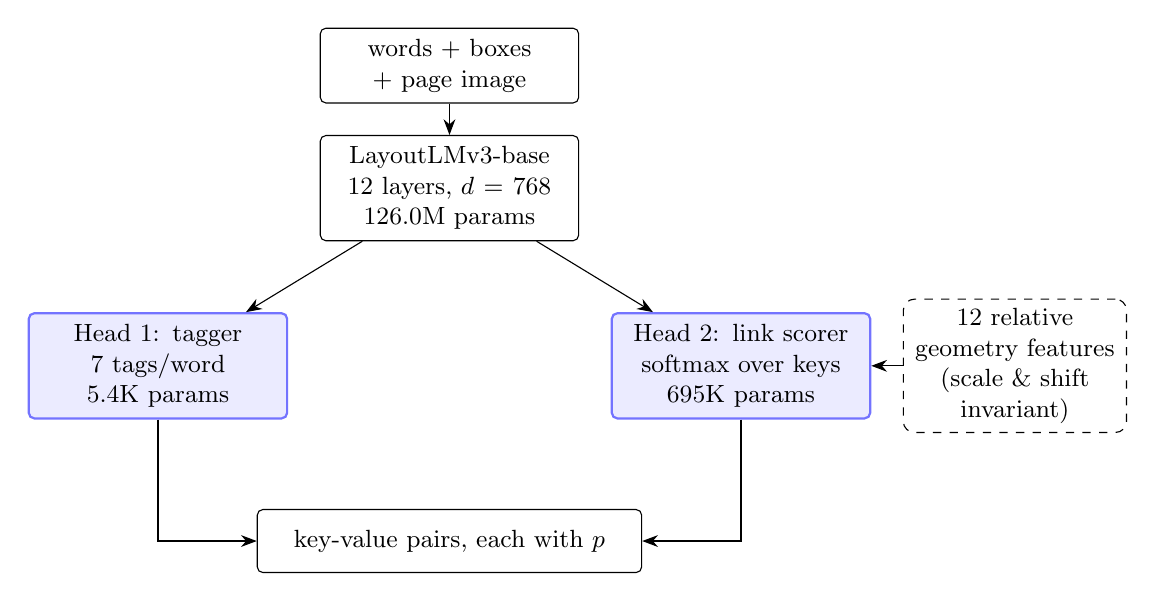
\begin{tikzpicture}[
  node distance=4mm,
  b/.style={draw,rounded corners=2pt,align=center,font=\small,inner sep=4pt,text width=30mm,minimum height=8mm},
  h/.style={b,fill=blue!8,draw=blue!55,thick},
  >={Stealth[length=2mm]}
]
\node[b] (in) {words + boxes\\+ page image};
\node[b,below=of in] (bb) {LayoutLMv3-base\\12 layers, $d=768$\\126.0M params};
\node[h,below left=9mm and 4mm of bb] (tag) {Head 1: tagger\\$7$ tags/word\\5.4K params};
\node[h,below right=9mm and 4mm of bb] (lnk) {Head 2: link scorer\\softmax over keys\\695K params};
\node[b,below=34mm of bb,text width=46mm] (out) {key-value pairs, each with $p$};
\node[draw,dashed,rounded corners,right=4mm of lnk,text width=26mm,font=\small,align=center]
     (geo) {12 relative geometry features (scale \& shift invariant)};
\draw[->] (in)--(bb);
\draw[->] (bb) -- (tag); \draw[->] (bb) -- (lnk);
\draw[->] (geo) -- (lnk);
\draw[->] (tag) |- (out); \draw[->] (lnk) |- (out);
\end{tikzpicture}
\caption{One backbone, two heads. Only the link head is geometry-invariant by construction; the
tagger sees LayoutLMv3's absolute coordinates and is regularised by augmentation instead.}
\label{fig:arch}
\end{figure}

\subsection{The interface}
\label{sec:interface}

The deliverable includes a web application so that the method can be exercised on a document the
model has never seen, rather than only through evaluation scripts. It is a Flask server started
with \code{python app\textbackslash app.py --run runs\textbackslash visual} and served at
\code{127.0.0.1:5000}.

\textbf{Methodology.} The design constraint is that the interface must run the \emph{same} code
path as the evaluation, so that what a user sees cannot diverge from what is reported. It
therefore imports the identical \code{kvx} modules: the same OCR wrapper, the same encoder, the
same checkpoint, the same decoding. Nothing is reimplemented for display. The model and the OCR
networks are loaded once at start-up and held resident; requests are served one at a time, because
a single GPU cannot safely run concurrent inference.

An upload is handled as follows. The file is accepted only if it is an image, a PDF, or one of the
annotation formats the loaders understand; anything else is rejected with HTTP 400 rather than
being guessed at. A PDF is rendered to page images at 144~dpi with \code{pypdfium2}. Each page
then goes through docTR, the chunker, the backbone and the two heads exactly as in
Section~\ref{sec:after}, and the resulting spans and links are serialised into a per-page payload
holding every word with its box, role and confidence; every predicted pair with its key box, value
box and link probability $p$; and the OCR and model timings.

\begin{table}[htbp]
\centering\small
\begin{tabular}{@{}p{3.1cm}p{10.3cm}@{}}
\toprule
\textbf{View} & \textbf{What it does} \\
\midrule
Extract & Accepts a dropped image or PDF and draws the extracted pairs on the rendered page.
Hovering a row highlights that key, that value and the link between them. A toggleable layer
colours every word by predicted role with per-role counts, which exposes tagger behaviour rather
than only the final pairs. Multi-page PDFs get page buttons. \\
Held-out examples & Serves pages the model was never trained on --- VRDU documents from unseen
templates, and seen-template test documents --- with every gold value marked found or missed by
the same matching function the metrics use, so the displayed verdict and the reported number
cannot disagree. \\
Results & Renders \code{metrics.json} from the evaluation run directly: seen versus unseen with
95\% intervals, the gap, per source and per field. It displays the measured file and computes
nothing of its own. \\
\bottomrule
\end{tabular}
\caption{The three views of the interface.}
\label{tab:interface}
\end{table}

The header reports which checkpoint, backbone, device and OCR models are live, and says so
explicitly when the PARSeq recogniser weights are absent and the cached CRNN fallback is in use ---
a silent fallback would otherwise make OCR quality look like model quality. Values that won no key
are listed as \code{(no key found)} rather than being dropped, which keeps the display honest
about what the model did and did not link.

%% ==================================================================== 5. DATA
\section{Data set Details}
\label{sec:data}

Four public corpora are used. Three train; one is held out entirely and is never trained on,
not even as unlabelled data.

\begin{table}[htbp]
\centering\small
\begin{tabular}{@{}llrrp{4.9cm}@{}}
\toprule
\textbf{Corpus} & \textbf{Role} & \textbf{Docs} & \textbf{Templates} & \textbf{Annotation} \\
\midrule
FUNSD        & train & 199   & 155   & entities typed question/answer/header \emph{and} links: full supervision \\
SROIE        & train & 973   & 307   & four field values per receipt; no keys, no links \\
WildReceipt  & train & 1{,}739 & 1{,}530 & 25 categories as \code{X\_key}/\code{X\_value}; links derived \\
VRDU         & \textbf{test only} & 2{,}556 & 1{,}100 & values only, with a type per field; no keys, no links \\
\bottomrule
\end{tabular}
\caption{The four corpora. VRDU contributes 4{,}991 annotated pages across its two corpora
(registration-form, 1{,}915 documents and 8{,}826 gold items; ad-buy-form, 641 documents and
14{,}149 gold items).}
\label{tab:data}
\end{table}

\textbf{Procurement.} All four are public research datasets, obtained from:

\begin{itemize}[leftmargin=1.4em,itemsep=0pt]
  \item FUNSD~\cite{funsd} --- \url{https://guillaumejaume.github.io/FUNSD/}
  \item SROIE~\cite{sroie}, ICDAR 2019 Robust Reading Challenge Task~3 ---
        \url{https://rrc.cvc.uab.es/?ch=13}
  \item WildReceipt~\cite{sdmgr}, distributed with MMOCR ---
        \url{https://download.openmmlab.com/mmocr/data/wildreceipt.tar}
  \item VRDU~\cite{vrdu}, Google Research ---
        \url{https://github.com/google-research-datasets/vrdu}
\end{itemize}

None is redistributed with our code; the repository documents these sources and the build scripts
consume whatever is placed in \code{data/}.

\textbf{Unified schema.} Every loader emits the same page-level record: a document id, a source
tag, the page image path and size, a list of words with their boxes, a list of entities with a
role and a span of word indices, and a list of links as (key entity, value entity) index pairs.
Optional fields record whether the page is fully annotated or value-only, the OCR line grouping,
words to ignore, and the gold field values used for field-level scoring. A validator refuses any
record with out-of-range boxes, dangling entity indices or links pointing at non-existent
entities, so a malformed corpus fails at build time rather than silently degrading training.

\textbf{Pre-processing.} Boxes are normalised to LayoutLMv3's $[0,1000]$ convention. Values in
value-only corpora are matched back onto the page's words by exact match first, then by a
normalised fuzzy match, so that a gold value \code{9.00} is found inside the printed
\code{RM9.00}. An alignment check rasterises a sample of pages and measures the share of boxes
containing ink against a deliberately shifted control, and reports \code{ALIGNED} only when the
real boxes contain substantially more ink than the control --- this catches coordinate-order
and origin errors that would otherwise look like model failure.

\textbf{Template induction.} None of the corpora ship template labels, so templates are induced.
Each page is reduced to a layout signature --- a coarse spatial histogram of its text boxes
together with the set of frequent short strings printed on it --- and pages are clustered by
average-linkage agglomerative clustering under a distance combining layout and text-set
dissimilarity. The threshold was fixed by inspecting FUNSD montages until clusters corresponded
to visually identical forms. The resulting counts appear in Table~\ref{tab:data}.

\textbf{The split.} Splitting is over \emph{templates}, not documents: a template's entire set of
documents goes to exactly one of train, validation, seen test and unseen test. Seen test holds
unseen \emph{documents} of training templates; unseen test holds documents of templates no
training document shares. After the split, assertions verify that no template id appears in more
than one of train, validation and unseen test, and a near-duplicate check verifies that no
held-out page lies within a small distance of any training page. These assertions run again
inside the training entry point, so a leak cannot survive to a reported number.

%% ============================================================== 6. EXPERIMENTS
\section{Experiments}
\label{sec:exp}

\textbf{Hardware and software.} A single NVIDIA GeForce RTX 5060 Laptop GPU under Windows 11,
with PyTorch 2.11 built against CUDA 12.8, bfloat16 automatic mixed precision, and Python 3.13.
One run of the no-image base configuration takes roughly two hours; a full evaluation over all three splits
takes about twenty minutes, and the VRDU benchmark scoring runs from saved predictions in about a
minute without loading the model.

\textbf{Training configuration.} LayoutLMv3-base backbone (126.0M parameters) plus 0.70M head
parameters; maximum 512 tokens per chunk with chunk boundaries placed only between units, so no
key or value is ever split; batch size 2 with gradient accumulation 2; AdamW with backbone
learning rate $3\times10^{-5}$, head learning rate $3\times10^{-4}$ and weight decay 0.01
excluding biases and LayerNorm; 10\% warmup then linear decay; gradient clipping at 1.0; up to 20
epochs with early stopping at patience 5 on the mean of the validation metrics. Sources are
sampled equally per epoch, so that WildReceipt's 1{,}231 training documents do not drown FUNSD's
126. The no-image base run selected epoch 16. The final model uses the identical configuration with
only \code{model.visual} switched on.

\subsection{Every experiment performed}

Table~\ref{tab:experiments} lists every configuration that was trained or scored during the
project, including the approach that was abandoned and the four ablations that remain unrun. Each
entry is one line of configuration away from the base run, which is what makes the comparisons in
Section~\ref{sec:ablations} interpretable.

\begin{table}[!htb]
\centering\small
\begin{tabular}{@{}p{3.6cm}lp{7.0cm}@{}}
\toprule
\textbf{Experiment} & \textbf{Status} & \textbf{Purpose / outcome} \\
\midrule
Query-based extractor & \textbf{negative; abandoned} & Section~\ref{sec:negative} \\
\code{runs\textbackslash base} & complete & the no-image baseline, and the reference for every ablation \\
\code{runs\textbackslash unseen15} & complete & holds out in-domain templates so that entity,
link and end-to-end F1 become measurable on unseen templates \\
\code{runs\textbackslash absgeom} & complete & absolute instead of relative link geometry \\
\code{runs\textbackslash noaug} & complete & augmentation disabled \\
\code{runs\textbackslash visual} & complete & \textbf{the reported system}: the LayoutLMv3 image stream enabled \\
VRDU through our own OCR & complete & tests the gold-OCR assumption \\
VRDU benchmark scoring & complete & re-scores saved predictions under VRDU's own protocol \\
\code{nogeom}, \code{nobalance}, \code{nosroie}, \code{segment} & not run & listed in
Section~\ref{sec:novelty} \\
\bottomrule
\end{tabular}
\caption{All experiments, including those that failed.}
\label{tab:experiments}
\end{table}

\subsection{Negative results}
\label{sec:negative}

\textbf{The query-based extractor failed and was abandoned.} Three measurements ended it. The
tag head \emph{collapsed on unseen templates}, scoring 0.019 on the FARA corpus while performing
acceptably on templates it had trained on --- the clearest possible symptom of template
memorisation. The candidate-pruning stage had a recall ceiling of 0.822, meaning that almost one
value in five was discarded before the model ever scored it, so no downstream improvement could
have recovered them. And the per-query formulation had no mechanism to disambiguate several
instances of one field type on a page. Focal loss on the tag head and a bounding-box anchor for
the query were implemented as remedies; the restart was taken before they could be evaluated
head to head, so we report them as unresolved rather than as fixes that did or did not work.
The lasting lesson is the one in Section~\ref{sec:before}: a query-based model must be told what
to ask for, which re-imposes the per-schema cost the project exists to remove.

\textbf{Augmentation is not measurably useful.} Disabling it changes nothing beyond noise
(Section~\ref{sec:ablations}). It is retained on argument, not evidence, and this is stated
rather than hidden.

\textbf{VRDU's ad-buy line items are effectively not extracted}, at 0.005 F1. This is a real
failure of the approach on tables and is analysed in Section~\ref{sec:limits}.

\textbf{A field-naming bug was found by inspecting test-set output.} Early VRDU scoring chose a
field by the longest matching alias, so a key reading ``Date of signature'' matched
\code{signer\_name} (via ``signature'', nine characters) in preference to \code{file\_date} (via
``date'', four), giving \code{file\_date} a recall of 0.144 against a value recall of 0.750. The
fix ranks candidate fields by whether the \emph{value}'s data type fits the field's matching
function before falling back to alias length. We record explicitly that this fix was motivated by
looking at test-set output, which is a form of test-set contact; any further mapping changes
belong on VRDU's own validation lists.

%% ================================================================= 7. RESULTS
\section{Results}
\label{sec:results}

\subsection{Metrics, and why some cells are empty}
\label{sec:metrics}

\begin{itemize}[leftmargin=1.4em,itemsep=1pt]
  \item \textbf{value\_recall} --- share of gold values the model produced as a value span
        anywhere on the page. Measurable on all four corpora, so it is the headline number.
  \item \textbf{kv\_field\_recall} --- value found \emph{and} linked to a key whose text maps to
        the right field name. Needs a field vocabulary: SROIE and VRDU only.
  \item \textbf{entity\_f1}, \textbf{link\_f1}, \textbf{e2e\_pair\_f1} --- span quality, linking
        quality given gold spans, and the two composed. All three need annotated keys and links:
        FUNSD and WildReceipt only.
\end{itemize}

VRDU and SROIE annotate values only. A metric those corpora cannot support is printed as
``--'', never as zero, because zero would be a claim about the model and ``--'' is a statement
about the data. All intervals are 95\% bootstrap intervals that resample \emph{templates}, since
documents of one template are not independent observations.

\subsection{The reported system against its no-image baseline}
\label{sec:reported}

The delivered model is the image-stream run (\code{runs\textbackslash visual}). Its baseline is
\code{runs\textbackslash base}, identical except that the image stream is off.
Table~\ref{tab:final} sets the two side by side on every measure available for both. Each is a
single run. Every table in this section and Figure~\ref{fig:perfield} describe the final model.
Where a no-image figure is given for comparison it is named explicitly. The \code{unseen15} run of
Section~\ref{sec:unseen15} and the \code{absgeom} and \code{noaug} ablations were trained with the
image stream off and are labelled as such throughout.

\begin{table}[htbp]
\centering\small
\begin{tabular}{@{}lcc@{}}
\toprule
\textbf{Measure} & \textbf{Final model (image on)} & \textbf{No-image base} \\
\midrule
Seen value recall                          & \textbf{0.928} & 0.918 \\
Unseen value recall (VRDU, pooled)         & \textbf{0.713} & 0.695 \\
Seen-minus-unseen gap                      & $\mathbf{+0.215}$ & $+0.223$ \\
Unseen value recall, registration-form     & \textbf{0.692} & 0.654 \\
Unseen value recall, ad-buy-form           & \textbf{0.720} & 0.709 \\
Registration-form micro F1 [95\% CI]       & 0.541 [0.454, 0.587] & \textbf{0.593} [0.567, 0.616] \\
Ad-buy-form unrepeated F1                  & \textbf{0.538} & 0.497 \\
Ad-buy-form macro F1                       & \textbf{0.453} & 0.420 \\
\bottomrule
\end{tabular}
\caption{The final model against its no-image baseline. Bold marks the better value in each row;
the gap row is better when smaller.}
\label{tab:final}
\end{table}

Value recall, the headline metric of Section~\ref{sec:metrics}, is higher with the image on in
every row that reports it: seen, unseen, and both held-out corpora. The pooled unseen figure is
dominated by ad-buy-form, which supplies 27{,}197 of the 36{,}026 unseen gold values, and that is
where the image helps most; registration-form supplies 8{,}829 and is where the image costs.
Section~\ref{sec:ablations} examines the two corpora separately and the field-level mechanism.

\subsection{Seen versus unseen templates}

\begin{table}[htbp]
\centering\small
\begin{tabular}{@{}lrrccccc@{}}
\toprule
\textbf{Split} & \textbf{Docs} & \textbf{Tmpl} & \textbf{value\_rec} &
\textbf{kv\_field\_rec} & \textbf{entity\_f1} & \textbf{link\_f1} & \textbf{e2e\_pair\_f1} \\
\midrule
val                & 310   & 197   & 0.950 & 0.754 & 0.932 & 0.936 & 0.802 \\
seen\_test         & 280   & 197   & 0.928 & 0.694 & 0.915 & 0.926 & 0.777 \\
unseen\_test (VRDU)& 4{,}991 & 1{,}100 & 0.713 & 0.495 & -- & -- & -- \\
\bottomrule
\end{tabular}
\caption{The final model (\code{runs\textbackslash visual}). Unseen test is VRDU in its entirety.}
\label{tab:main}
\end{table}

\begin{table}[htbp]
\centering\small
\begin{tabular}{@{}lccrcr@{}}
\toprule
\textbf{Metric} & \textbf{Seen} & \textbf{Unseen} & \textbf{Gap} & \textbf{95\% CI} &
\textbf{Relative drop} \\
\midrule
value\_recall    & 0.928 & 0.713 & $+0.215$ & $[+0.185, +0.240]$ & 23.2\% \\
kv\_field\_recall& 0.694 & 0.495 & $+0.199$ & $[+0.090, +0.318]$ & 28.7\% \\
\bottomrule
\end{tabular}
\caption{The generalisation gap of the final model. The value-recall gap is narrower than the
no-image run's $+0.223$, but the \code{kv\_field\_recall} gap is \emph{wider} ($+0.137$ for the
no-image run): the image stream finds more values on unseen templates and names a smaller share
of them.}
\label{tab:gap}
\end{table}

\subsection{Separating template novelty from domain novelty}
\label{sec:unseen15}

Table~\ref{tab:main} cannot fill its last three columns because every held-out template comes
from VRDU. Re-splitting with 15\% of FUNSD and WildReceipt templates held out and retraining
(\code{runs\textbackslash unseen15}, trained without the image stream) fills them, and the result is the most important in this
report.

\begin{table}[htbp]
\centering\small
\begin{tabular}{@{}lccrcr@{}}
\toprule
\textbf{Metric} & \textbf{Seen} & \textbf{Unseen} & \textbf{Gap} & \textbf{95\% CI} &
\textbf{Relative} \\
\midrule
value\_recall     & 0.918 & 0.728 & $+0.189$ & $[+0.153, +0.220]$ & 20.6\% \\
kv\_field\_recall & 0.711 & 0.479 & $+0.233$ & $[+0.114, +0.354]$ & 32.7\% \\
entity\_f1        & 0.897 & 0.913 & $-0.016$ & $[-0.054, +0.020]$ & $-1.8$\% \\
link\_f1          & 0.949 & 0.942 & $+0.007$ & $[-0.023, +0.037]$ & 0.7\% \\
e2e\_pair\_f1     & 0.788 & 0.778 & $+0.010$ & $[-0.068, +0.097]$ & 1.2\% \\
\bottomrule
\end{tabular}
\caption{The \code{unseen15} run. \textbf{All three structural metrics have gap intervals
containing zero}: they do not degrade on unseen templates.}
\label{tab:unseen15}
\end{table}

Only the two recall metrics fall, and the per-source rows locate the fall:

\begin{table}[htbp]
\centering\small
\begin{tabular}{@{}lcc@{}}
\toprule
\textbf{Source} & \textbf{Seen value recall} & \textbf{Unseen value recall} \\
\midrule
FUNSD        & 0.894 (20 docs)  & 0.894 (32 docs) \\
WildReceipt  & 0.971 (69 docs)  & 0.975 (261 docs) \\
SROIE        & 0.813 (142 docs) & 0.780 (146 docs) \\
VRDU-FARA    & --               & 0.681 (3{,}632 docs) \\
VRDU-DeepForm& --               & 0.689 (1{,}359 docs) \\
\bottomrule
\end{tabular}
\caption{Within a source, unseen templates cost almost nothing.}
\label{tab:persource}
\end{table}

FUNSD is identical to three decimal places; WildReceipt is marginally better on unseen
templates; SROIE loses 3.3 points. The aggregate gap of 0.189 is an artefact of composition,
because 4{,}991 of the 5{,}430 unseen documents are VRDU, a domain with no training
representation at all. \textbf{Template novelty is close to free; domain novelty is what costs.}
The error breakdown agrees: 94.6\% of gold-linked values take the right key on seen templates and
94.4\% on unseen ones.

\subsection{VRDU benchmark-style field scores}

Re-scoring the saved predictions under VRDU's own type-specific matching and its
precision/recall/F1 definition, with no VRDU training data of any kind, gives the final model
\textbf{0.541 micro F1} on registration-form (CI $[0.454, 0.587]$) and \textbf{0.538 unrepeated
F1} on ad-buy-form (macro F1 0.453). The no-image base run, scored the same way, gives 0.593 micro
F1 on registration-form (micro P 0.656, R 0.541, CI $[0.567, 0.616]$) and 0.497 unrepeated F1 on
ad-buy-form. Per field, the final model reaches 0.888 F1 on \code{registration\_num} and 0.560 on
\code{registrant\_name} (0.920 and 0.789 in the no-image run), while \code{signer\_title} scores
0.000 and \code{line\_item} 0.005.

The \code{unseen15} run of Section~\ref{sec:unseen15}, which also has the image off, scores lower
on the same metric --- 0.516 micro F1 $[0.437, 0.542]$ on registration-form and 0.456 unrepeated
F1 on ad-buy-form --- which is the expected cost of the 377 training documents it gives up in
order to make the structural metrics measurable. The runs answer different questions:
\code{runs\textbackslash visual} is the delivered system, \code{runs\textbackslash base} its
no-image baseline, and \code{unseen15} the instrument that separates template novelty from domain
novelty.

\subsection{Per-field behaviour: finding is not keying}

\begin{figure}[!htb]
\centering
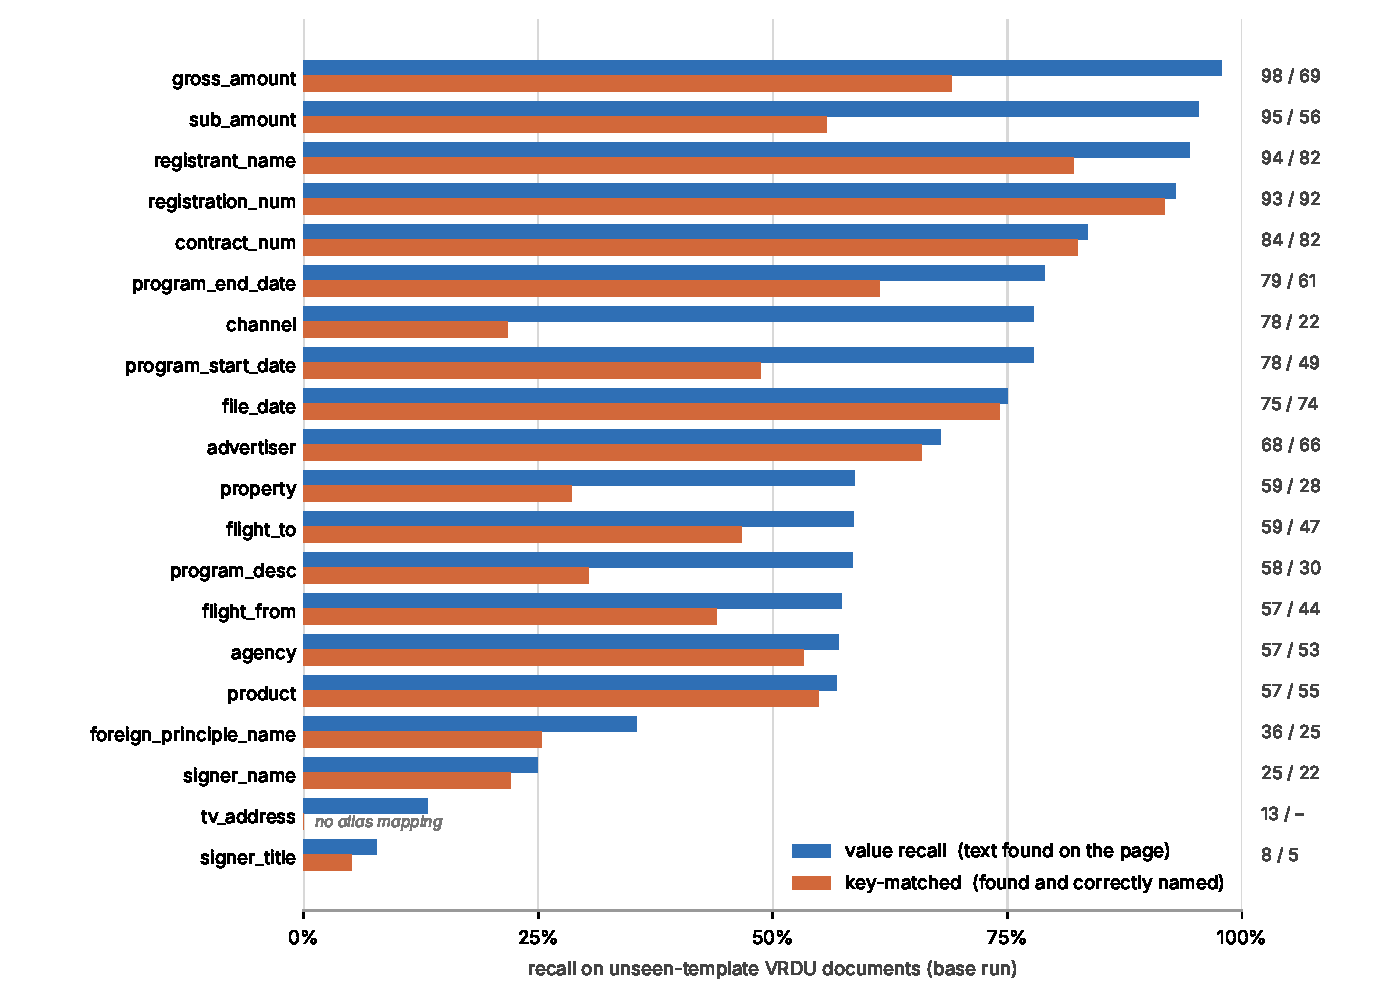
\includegraphics[width=0.90\textwidth]{perfield.pdf}
\caption{VRDU per-field recall on unseen templates, final model (image stream on), both corpora
pooled. The upper bar is value recall (the text was found); the lower bar is key-matched recall
(found \emph{and} correctly named). The distance between them is the share of values the model
located but could not name. \code{tv\_address} has no alias mapping and so has no key-matched bar.}
\label{fig:perfield}
\end{figure}

Three bands are visible in Figure~\ref{fig:perfield}. Fields with one stable printed label ---
\code{registration\_num} (88/87), \code{contract\_num} (82/82), \code{file\_date} (76/76),
\code{advertiser} (75/70) --- have bars within five points of each other: once found, they are
named correctly. Table columns collapse: \code{channel} falls from 0.787 to 0.250,
\code{sub\_amount} from 0.867 to 0.462, \code{gross\_amount} from 0.959 to 0.738. Values with no
printed label at all are never found in the first place: \code{signer\_title} 0.084,
\code{tv\_address} 0.251, \code{signer\_name} 0.351.

\subsection{Ablations}
\label{sec:ablations}

Every row of Table~\ref{tab:ablations} is one configuration key away from the no-image base run.
The \code{absgeom} and \code{noaug} runs were trained with the image stream off, so their effects
are measured on the no-image configuration and were not repeated on the final model. The
\code{visual} row is the final model.

\begin{table}[htbp]
\centering\small
\begin{tabular}{@{}lccrcc@{}}
\toprule
\textbf{Run} & \textbf{Seen} & \textbf{Unseen} & \textbf{Gap} &
\textbf{FARA F1 [95\% CI]} & \textbf{DeepForm F1} \\
\midrule
base (no image)                       & 0.918 & 0.695 & $+0.223$ & \textbf{0.593} $[0.567, 0.616]$ & \textbf{0.497} \\
\code{absgeom} (absolute geometry)    & \textbf{0.938} & 0.671 & $+0.267$ & 0.541 $[0.452, 0.593]$ & 0.484 \\
\code{noaug} (no augmentation)        & 0.933 & 0.703 & $+0.230$ & 0.571 $[0.524, 0.608]$ & 0.478 \\
\code{visual} (image on, final)       & 0.928 & \textbf{0.713} & $\mathbf{+0.215}$ & 0.541 $[0.454, 0.587]$ & \textbf{0.538} \\
\bottomrule
\end{tabular}
\caption{Ablations. The base run uses relative geometry and augmentation with the image stream off; the \code{visual} row adds the image stream and is the final model. Seen and unseen columns are value recall.}
\label{tab:ablations}
\end{table}

\textbf{\code{absgeom} moves every measure in the predicted direction.} Absolute geometry is
\emph{better} than relative geometry on seen templates --- 0.938 against 0.918 value recall ---
and worse on every measure that involves a template the model has not met: unseen value recall
falls from 0.695 to 0.671, the seen-minus-unseen gap widens from $+0.223$ to $+0.267$, the FARA
field score drops from 0.593 to 0.541, and the DeepForm score from 0.497 to 0.484. Five
independent measures, one direction. The natural reading is that absolute coordinates buy
in-domain accuracy by learning where fields sit on the training templates, which is precisely the
shortcut the relative frame is designed to remove; an ablation that merely removed capacity would
have cost accuracy on both sides rather than trading one for the other.

\textbf{No single one of those differences is statistically significant, and the report does not
claim otherwise.} The FARA intervals $[0.567, 0.616]$ and $[0.452, 0.593]$ overlap, as do the two
gap intervals $[+0.188, +0.253]$ and $[+0.238, +0.298]$. With one run per configuration and
bootstrap intervals taken over templates, this experiment can establish a consistent direction but
not significance; distinguishing the two would need several seeds per configuration, which was
beyond the compute available. The honest summary is that the geometry result is
\emph{directionally consistent across five measures and two corpora, and individually
inconclusive on each}.

\textbf{\code{noaug} is weaker still.} Its FARA interval $[0.524, 0.608]$ sits almost entirely
inside the base interval, and unseen value recall is in fact marginally \emph{higher} without
augmentation (0.703 against 0.695). Scale, shift and jitter make no measurable difference on this
test set. They cost nothing and are kept on the argument given in Section~\ref{sec:after} rather
than on evidence, and that is a weaker footing than the geometry claim.

\textbf{\code{visual} did not behave as predicted, and the result is the most surprising in the
project.} The expectation, by analogy with \code{absgeom}, was that the page image would help
in-domain and hurt on unseen templates, because appearance is highly template-specific. Instead it
improved \emph{both}: seen value recall 0.928 against 0.918, unseen 0.713 against 0.695, and a gap
of $+0.215$ that is marginally narrower rather than wider. Both held-out corpora gained
independently (FARA 0.654 $\to$ 0.692, DeepForm 0.709 $\to$ 0.720), so it is not one corpus
carrying the result.

The field-level picture is split, and that is where the mechanism shows. On \textbf{ad-buy-form}
the image stream is clearly better --- unrepeated F1 0.538 against 0.497, macro F1 0.453 against
0.420, with \code{advertiser} rising from 0.548 to 0.628 and \code{contract\_num} from 0.577 to
0.643. On \textbf{registration-form} it is clearly worse --- 0.541 against 0.593, driven almost
entirely by \code{registrant\_name} collapsing from 0.789 to 0.560. The gains concentrate on
fields with weak or absent printed labels (\code{foreign\_principle\_name} value recall 0.352
$\to$ 0.568, \code{agency} 0.572 $\to$ 0.738, \code{tv\_address} 0.138 $\to$ 0.251), which is what
one would expect: where no text names a value, appearance is the only remaining cue, and the
text-only model is blind there. The losses concentrate on text-dense government forms where a
printed label already identifies the field and the image adds nothing but a template-specific
distraction.

The honest summary is that the page image is \emph{not} simply another shortcut of the kind
absolute coordinates provided. It buys genuine recall on visually structured documents and costs
precision on textually labelled ones.

\textbf{Decision.} The image-stream configuration is the delivered model. The deciding measure is
the headline one of Section~\ref{sec:metrics}, value recall. With the image on it is higher on
seen templates (0.928 against 0.918), higher on unseen templates (0.713 against 0.695), higher on
both held-out corpora, and the seen-minus-unseen gap is slightly narrower. The configuration also
scores higher on ad-buy-form, which supplies three quarters of the unseen gold values (27{,}197 of
36{,}026). Against this stands a real cost: registration-form F1 falls from 0.593 to 0.541, with
\code{registrant\_name} collapsing, and the run's registration-form interval
($[0.454, 0.587]$ against $[0.567, 0.616]$) is markedly wider. Those intervals overlap, each
configuration is a single run, and so the report claims a direction on the headline metric and
not a significant improvement; several seeds per configuration would be needed to settle it. The
no-image checkpoint \code{runs\textbackslash base} is released alongside the final model for
anyone who weights registration-form precision above recall on label-poor fields.

\subsection{Qualitative results}

Numbers alone do not show whether a prediction is sensible, so three artefacts are produced
alongside them. Step~3 renders gold annotations onto sample pages, which is how the template
clustering threshold was fixed by eye. Step~5 writes a \code{qualitative/} directory per run
holding predicted pages with key and value boxes drawn and each link joined, sampled from both the
seen and the unseen splits. Step~6 writes an \code{errors/} directory containing the individual
failure cases behind each error category in the tables above, so that a claim such as ``wrong key,
nearer than gold'' can be checked against the page that produced it.

The interface of Section~\ref{sec:interface} is the interactive form of the same thing: its
held-out examples view marks every gold value found or missed on documents from unseen templates,
using the same matching function as the metrics, and its extract view shows the model's output on
a document supplied by the user.

\subsection{Failure analysis: what limits generalisation}
\label{sec:limits}

\textbf{Scope.} The failure analysis consists of error bucketing on seen templates, counterfactual
probes, and value recall stratified by structural properties of the gold value. The analysis files
used for this report were produced from the final model (\code{runs\textbackslash visual}); where a
no-image figure is given for comparison it is named. Four of the seven probes --- \code{identity},
\code{shift\_scale}, \code{mirror\_x} and \code{reading\_order} --- carry the page image edited
consistently with the geometry, so the model keeps the input it was trained with. The remaining
three move or mask individual entities, which the pixels cannot follow, and so run on a blank page;
they are marked in Table~\ref{tab:probes} and should be read only against each other and against
the identity row.

\textbf{On seen templates linking is rarely the problem.} Of 1{,}098 gold-linked values, 1{,}045
(95.2\%) take the right key. The remainder split into 21 wrong keys that were nearer than the
gold key (1.9\%), 21 wrong keys that were not nearer (1.9\%), and 11 values given no key (1.0\%);
20 of 1{,}376 keyless values (1.5\%) were wrongly given a key. The two wrong-key types suggest
different causes: proximity winning over the right key in the first case, and key text outweighing
distance in the second. The larger error source is tagging. At word level 95.9\% of gold value
words are tagged as values, but 285 words that are not values are (12.1\% of the \code{O} words;
value precision 91.7\%), and 136 value words are missed. Keys are recovered at 90.6\% (88 lost to
\code{O}, 48 mistaken for values), and 50 of 242 header words (20.7\%) are called keys. Only 117
of 5{,}691 tagged words (2.1\%) have the right role with the wrong B/I prefix.

Every one of those linking figures is marginally \emph{worse} than the no-image run's, which
scores 96.3\% correct with 14 nearer-key errors and 6 no-key predictions, and recovers keys at
91.3\%. Stratified by source the same small regression appears: link recall falls from 0.966 to
0.954 on FUNSD and from 0.962 to 0.953 on WildReceipt, and from 0.968 to 0.960 on one-to-one keys.
This is the seen-template counterpart of the \code{registrant\_name} cost in
Section~\ref{sec:ablations}: the image stream buys unseen value recall and gives back a little
seen-template linking accuracy.

\textbf{Counterfactual probes.} Each probe edits one property of a fully annotated seen-test page
and re-runs the model. Every probe is read against the identity row of its own table, not against
the evaluation report: on the held-out documents the identity row is 0.724 against 0.713 in the
evaluation, the difference being the 60-page probe sample.

\begin{table}[htbp]
\centering\small
\begin{tabular}{@{}lccccc@{}}
\toprule
\textbf{Probe} & \textbf{value recall} & \textbf{value acc.} & \textbf{link F1} & \textbf{entity F1} & \textbf{pair F1} \\
\midrule
identity                    & 0.941 & 0.953 & 0.925 & 0.890 & 0.737 \\
\code{shift\_scale}         & 0.932 & 0.958 & 0.930 & 0.890 & 0.736 \\
\code{mirror\_x}            & 0.888 & 0.773 & 0.760 & 0.820 & 0.510 \\
\code{value\_below}$^\dagger$     & 0.883 & 0.758 & 0.732 & 0.842 & 0.521 \\
\code{value\_right}$^\dagger$     & 0.908 & 0.963 & 0.932 & 0.863 & 0.683 \\
\code{key\_text\_masked}$^\dagger$& 0.852 & 0.760 & 0.797 & 0.493 & 0.011 \\
\code{reading\_order}       & 0.931 & 0.953 & 0.925 & 0.850 & 0.654 \\
\bottomrule
\end{tabular}
\caption{Counterfactual probes on fully annotated seen-test documents, final model. Rows without a
dagger carry the page image edited to match the geometry; $^\dagger$ marks the three probes that
run on a blank page, because the pixels cannot follow a per-entity move. On the held-out VRDU
documents only value recall is measurable: identity 0.724, \code{shift\_scale} 0.671 ($-0.053$),
\code{mirror\_x} 0.615 ($-0.108$).}
\label{tab:probes}
\end{table}

Three readings follow from Table~\ref{tab:probes}. First, a \emph{direction prior}: mirroring the
page costs 0.180 of value accuracy and 0.165 of link F1, and moving every value below its key
costs 0.195 and 0.193, while moving every value to the right of its key \emph{improves} value
accuracy (+0.010) and link F1 (+0.007). The model has learned that values sit to the right of
their keys. Second, \emph{the invariance proof holds, and on the final model the residue is gone}:
under shift and scale the link F1 \emph{rises} slightly, 0.925 to 0.930, entity F1 is unchanged at
0.890 and pair F1 moves by 0.001, while value recall falls by 0.009. The no-image run showed a
larger residue (value recall $-0.017$, entity F1 $-0.008$, pair F1 $-0.017$), attributed there to
the tagger seeing LayoutLMv3's absolute coordinates. With the page image transformed consistently
with the boxes that residue all but disappears, which suggests part of it was the tagger losing
positional grounding rather than depending on absolute coordinates alone. On the held-out
documents, where the image is also edited, value recall falls by 0.053 under shift and scale and
0.108 under mirroring: mirroring the pixels as well as the boxes is a larger perturbation than
mirroring boxes alone. Third, \emph{key text matters most for finding keys}: masking every key's
text roughly halves entity F1 (0.890 to 0.493) and takes pair F1 from 0.737 to 0.011, while link
F1 given the spans falls less (0.925 to 0.797). Perturbing the reading order leaves link F1
untouched (0.925) but costs entity F1 0.040 and pair F1 0.083, so span recognition, not linking,
depends on token order.

\textbf{Held-out value recall by structure.} Table~\ref{tab:strata} stratifies value recall on
the 36{,}026 unseen gold values by structural properties of the value.

\begin{table}[htbp]
\centering\small
\begin{tabular}{@{}llrc@{}}
\toprule
\textbf{Property} & \textbf{Bucket} & \textbf{n} & \textbf{Value recall} \\
\midrule
Lines          & single-line      & 32{,}710 & 0.746 \\
               & multi-line       & 3{,}316  & 0.390 \\
Words          & 1 word           & 19{,}991 & 0.784 \\
               & 2--4 words       & 11{,}635 & 0.661 \\
               & 5+ words         & 4{,}400  & 0.532 \\
Structure      & single field     & 18{,}236 & 0.662 \\
               & table line item  & 17{,}790 & 0.765 \\
Page           & first page       & 18{,}129 & 0.744 \\
               & later page       & 17{,}897 & 0.682 \\
Vertical       & top third        & 15{,}643 & 0.672 \\
               & middle third     & 13{,}691 & 0.788 \\
               & bottom third     & 6{,}689  & 0.657 \\
\bottomrule
\end{tabular}
\caption{Unseen-template value recall by structural property of the gold value, final model. By
value type, recall is 0.870 for date-like, 0.710 for mixed, 0.662 for alphabetic and 0.615 for
numeric values.}
\label{tab:strata}
\end{table}

Two structural assumptions fail, and the failure analysis names both.

\textbf{``A key sits beside its value'' fails for tables.} A column header is one key for dozens
of values stacked beneath it, which is not the one-key-beside-one-value geometry the link scorer
was trained on. This produces the found-but-not-keyed collapse of Figure~\ref{fig:perfield} and
the 0.005 line-item F1. Table cells are in fact \emph{found}: value recall on table line items is
0.765, higher than the 0.662 on single fields. What fails is attaching them to a header and
assembling them into rows. The probes agree on the cause. A key serving many values is not itself
the problem, since on seen templates one-to-many keys score 0.947 against 0.960 for one-to-one;
the direction is, because a header sits \emph{above} its values and moving every value below its
key costs 0.195 of value accuracy. Stratifying by the direction from key to value on seen
templates points the same way: recall is 0.976 for values to the right of their key and 0.979 for
values below, but 0.444 for other diagonals and 0.833 for values to the left. Those last two
buckets hold only 27 and 12 values, which the analysis itself treats as anecdotal.

\textbf{``Every value has a printed label'' fails for signature and address blocks.} Here the
first bar is already low --- the tagger does not mark the span at all --- because nothing on the
page says what the text is: \code{signer\_title} 0.084, \code{tv\_address} 0.251,
\code{signer\_name} 0.351. The same failure appears on seen templates, where the SROIE
\code{company} field, a receipt's header with no printed label, has value recall 0.549 against
1.000 for \code{total}, and where \code{date} is found 0.902 of the time but matched to a key only
0.482. A schema-free model cannot invent a field name, so for text-only evidence this is an honest
ceiling of the approach rather than a tuning gap. Masking all key text drives end-to-end pair F1
to 0.011, confirming how much of the decision rests on what keys say.

A third, softer limit is multi-line and long values: recall falls from 0.746 on single-line
values to 0.390 on multi-line ones, and from 0.784 on one-word values to 0.532 on values of five
words or more. Seen templates hold only 24 multi-line values, too few to say whether the drop
there is as steep.

\textbf{What the image stream changes.} Two measurements locate its effect. Per field, its gains
sit on exactly the fields the analysis above calls label-poor:
\code{foreign\_principle\_name} value recall rises from 0.352 to 0.568, \code{agency} from 0.572
to 0.738 and \code{tv\_address} from 0.138 to 0.251. So the second assumption's ceiling is a
ceiling for text and geometry only; appearance supplies a cue where no text names the value, but
the lift is partial, and \code{tv\_address} is still at 0.251.

Structurally, comparing the two runs over the same 36{,}026 unseen gold values, the gains
concentrate on \emph{long and multi-line} values: multi-line recall rises from 0.270 to 0.390 and
five-or-more-word values from 0.400 to 0.532, with two-to-four-word values from 0.594 to 0.661. It
\emph{costs} on short ones --- single-word values fall from 0.819 to 0.784, numeric from 0.632 to
0.615 and date-like from 0.895 to 0.870. The natural reading is that appearance tells the tagger
where a span \emph{ends}: ruling lines, cell boundaries and blocks of whitespace delimit a
multi-line address or a long programme description in a way text alone cannot, so fewer such spans
are truncated. Where the value is a single token the text already settled the question and the
pixels only add noise. That is the same shape as the losses, which sit on text-dense registration
forms where \code{registrant\_name} F1 falls from 0.789 to 0.560 even though a printed label
already identifies the field, and on seen-template linking, which gives back about a point. Taken
together the two measurements give one account of the image stream: \emph{it helps wherever the
textual evidence is weak}, whether because no printed label names the value or because nothing in
the text marks where it stops, and it costs a little wherever the text already settles the matter.
The mechanism is an interpretation of the per-field and structural breakdowns; no per-document
inspection has tested it. Still not measured: the three per-entity probes on an edited image,
which would need a page image consistent with a moved or masked entity.

%% ================================================================= 8. NOVELTY
\section{Plan for Novelty Assessment}
\label{sec:novelty}

The failure analysis points at three changes that are principled rather than tuning, in that each
targets a named structural assumption and uses machinery the model already has.

\begin{enumerate}[leftmargin=1.5em,itemsep=2pt]
  \item \textbf{Group table cells into rows by vertical banding rather than reading order.}
        Targets the 0.005 line-item F1. Reading-order grouping breaks whenever one cell is missing
        or extra; banding by shared vertical position is how a person reads a table row.
  \item \textbf{Allow a key above a column of values}, weighting the column-overlap feature
        accordingly. Targets the found-but-not-keyed collapse. The geometry features already carry
        horizontal overlap; the training data simply contains very few table examples, so the
        relation is never learned.
  \item \textbf{Permit a value whose nearest label sits \emph{below} it}, as in signature blocks.
        Targets \code{signer\_title} at 0.078. The direction features exist and nothing in the
        model forbids this; it was never taught.
\end{enumerate}

All three must be developed against the in-domain unseen split or VRDU's own validation lists,
never against the VRDU test documents reported here. Alongside them, four ablations remain
unrun --- \code{nogeom} (is linking carried by geometry or by key text?), \code{nobalance} (does
equal source sampling matter?), \code{nosroie} (does value-only supervision help at all?) and
\code{segment} (how optimistic is the gold-segment box protocol against honest per-word boxes?).
Two further items follow from the choice of final model: several seeds per configuration, to
separate the image stream's effect from run-to-run noise, and probe images that are edited
consistently with a \emph{moved or masked entity}, which would extend the image-consistent probing
already done for \code{identity}, \code{shift\_scale}, \code{mirror\_x} and \code{reading\_order}
to the remaining three.

%% ============================================================== 9. CONCLUSION
\section{Conclusion}
\label{sec:conclusion}

We built a schema-free key-value extraction system that is told nothing about which fields a form
contains, and evaluated it under a template-level split with explicit leakage assertions. On
templates it has never seen, the final model recovers 0.713 of gold values against 0.928 on seen
templates, and under VRDU's own benchmark-style field metric scores 0.541 micro F1 on
registration forms and 0.538 unrepeated F1 on ad-buy forms, with no VRDU training data of any
kind.

Four conclusions are supported by the measurements rather than by argument.

\textbf{Relative geometry appears to be what makes the representation transfer.} The
\code{absgeom} ablation scores \emph{better} than the no-image base system on seen templates and worse on
every cross-template measure --- unseen value recall, the width of the gap, and both VRDU corpora.
That asymmetry is the signature of a removed shortcut rather than of reduced capacity. The
intervals overlap, so the result is directionally consistent across five measures rather than
individually significant; confirming it would need several seeds per configuration. Both the
geometry and the augmentation ablations were run with the image stream off, and were not
repeated on the final model.

\textbf{Template novelty is nearly free; domain novelty is the real cost.} Under a split that
holds out in-domain templates, entity F1, link F1 and end-to-end pair F1 show no degradation at
all --- every gap interval contains zero (measured on the no-image configuration) --- while value recall falls only on the cross-domain
VRDU documents. The headline gap (0.223 for the no-image run, 0.215 for the final model) is therefore a statement about domain shift, and
reading it as a template-generalisation gap would be wrong.

\textbf{The page image helps the headline metric, but not uniformly.} With the image stream on,
value recall rises on seen and unseen templates and on both held-out corpora, and the gains
concentrate on fields with weak or absent printed labels. Registration-form F1 falls, driven by
one field. This is the basis for making it the final model, and it rests on a single run.

\textbf{The failure modes are structural and nameable.} The model assumes a key sits beside its
value and that every value carries a printed label. Tables break the first; signature and address
blocks break the second. Both were identified by counterfactual probes rather than by inspection.

Future work follows directly: the three changes in Section~\ref{sec:novelty}, the four remaining
ablations, several seeds per configuration, probe images edited consistently with a moved or masked
entity, and an evaluation on forms from a third domain to test whether the domain-shift conclusion
holds beyond VRDU.

%% ============================================================== REFERENCES
\begin{thebibliography}{9}\small

\bibitem{layoutlm} Yiheng Xu, Minghao Li, Lei Cui, Shaohan Huang, Furu Wei, and Ming Zhou.
\emph{LayoutLM: Pre-training of Text and Layout for Document Image Understanding}, KDD, 2020.
\url{https://arxiv.org/abs/1912.13318}

\bibitem{layoutlmv2} Yang Xu, Yiheng Xu, Tengchao Lv, Lei Cui, and Furu Wei.
\emph{LayoutLMv2: Multi-modal Pre-training for Visually-rich Document Understanding}, ACL, 2021.
\url{https://arxiv.org/abs/2012.14740}

\bibitem{layoutlmv3} Yupan Huang, Tengchao Lv, Lei Cui, Yutong Lu, and Furu Wei.
\emph{LayoutLMv3: Pre-training for Document AI with Unified Text and Image Masking},
ACM Multimedia, 2022. \url{https://arxiv.org/abs/2204.08387}

\bibitem{funsd} Guillaume Jaume, Hazim Kemal Ekenel, and Jean-Philippe Thiran.
\emph{FUNSD: A Dataset for Form Understanding in Noisy Scanned Documents}, ICDAR-OST, 2019.
\url{https://arxiv.org/abs/1905.13538}

\bibitem{sroie} Zheng Huang, Kai Chen, Jianhua He, Xiang Bai, Dimosthenis Karatzas, Shijian Lu,
and C. V. Jawahar. \emph{ICDAR2019 Competition on Scanned Receipt OCR and Information
Extraction}, ICDAR, 2019. \url{https://rrc.cvc.uab.es/?ch=13}

\bibitem{sdmgr} Hongbin Sun, Zhanghui Kuang, Xiaoyu Yue, Chenhao Lin, and Wayne Zhang.
\emph{Spatial Dual-Modality Graph Reasoning for Key Information Extraction}, arXiv preprint,
2021. \url{https://arxiv.org/abs/2103.14470} (Introduces the WildReceipt dataset.)

\bibitem{vrdu} Zilong Wang, Yichao Zhou, Wei Wei, Chen-Yu Lee, and Sandeep Tata.
\emph{VRDU: A Benchmark for Visually-rich Document Understanding}, KDD, 2023.
\url{https://arxiv.org/abs/2211.15421}

\bibitem{doctr} Mindee. \emph{docTR: Document Text Recognition}, open-source library, 2021.
\url{https://github.com/mindee/doctr}. Accessed on: 25th October, 2026.

\bibitem{fast} Zhe Chen, Jiahao Wang, Wenhai Wang, Guo Chen, Enze Xie, Ping Luo, and Tong Lu.
\emph{FAST: Faster Arbitrarily-Shaped Text Detector with Minimalist Kernel Representation},
arXiv preprint, 2021. \url{https://arxiv.org/abs/2111.02394}

\bibitem{parseq} Darwin Bautista and Rowel Atienza.
\emph{Scene Text Recognition with Permuted Autoregressive Sequence Models}, ECCV, 2022.
\url{https://arxiv.org/abs/2207.06966}

\end{thebibliography}

\end{document}
